\documentclass[a4paper]{eccomas_paper-2024}

\usepackage{graphicx}
\usepackage{hyperref}
\usepackage{amsmath}
\usepackage{amsfonts}
\usepackage{amssymb}

\title{INSTRUCTIONS TO PREPARE A FULL PAPER FOR THE 9th EUROPEAN CONGRESS ON COMPUTATIONAL METHODS IN APPLIED SCIENCES AND ENGINEERING\break ECCOMAS CONGRESS 2024}

\author{FIRST A. AUTHOR$^1$, SECOND B. AUTHOR$^2$ AND THIRD C. AUTHOR$^1$}

\heading{First A. Author, Second B. Author and Third C. Author}

\address{$^{1}$ International Center for Numerical Methods in Engineering (CIMNE)\\
Universidad Polit\'{e}cnica de Catalu\~{n}a\\
Campus Norte UPC, 08034 Barcelona, Spain\\
e-mail: congress@cimne.upc.edu, www.cimne.com
\and
$^{2}$ Spanish Association for Numerical Methods in Engineering (SEMNI)\\
Edificio C1, Campus Norte UPC\\
Gran Capit\'{a}n s/n, 08034 Barcelona, Spain\\
email: semni@cimne.upc.edu, www.semni.org
}

\keywords{Computational Mechanics, FEM, Contact Problems}

\abstract{This document provides information and instructions for
preparing a Full Paper to be included in the Proceedings
of {\it ECCOMAS CONGRESS 2024}. }

\begin{document}
\thispagestyle{empty}

\section{INTRODUCTION}

All the participants whose Abstract has been accepted for presentation at the ECCOMAS 2022 Congress are kindly requested to submit the Full Paper electronically via the web page of the \href{https://eccomas2024.org/lisbon}{Congress}, before \textbf{July 1st, 2024}. Congress Proceedings (including full papers only) will be published on Scipedia with DOI number after the congress and will be submitted for indexation to SCOPUS database. Submission of the full paper is not mandatory. The Full Paper should be written following the format of macros for submission. The file has to be translated into Portable Document Format (PDF) before submission via the Conference site. The organizers do not commit themselves to include in the Proceedings any Full Paper received later than the above-mentioned deadline. The corresponding author should be the speaker, and is expected to register and pay his registration fee during the advance period (before \textbf{April 1st, 2024}) for the paper to be included in the technical programme of the ECCOMAS 2024.

\section{METHODS}

\section{RESULTS}

\subsection{Problem setup}

\begin{figure}
    \begin{center}
        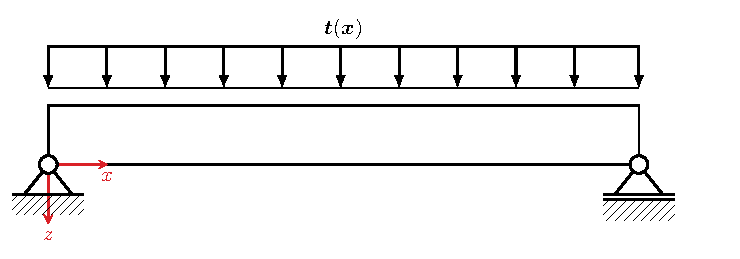
\includegraphics[width=0.95\textwidth]{../figures/beam/beam_sketch.pdf}
    \end{center}
    \caption{Schematic representation of the structural problem. A simply supported beam is subjected to a constant load.}\label{fig:beam_sketch}
\end{figure}

% TODO placement
\begin{figure}
    \begin{center}
        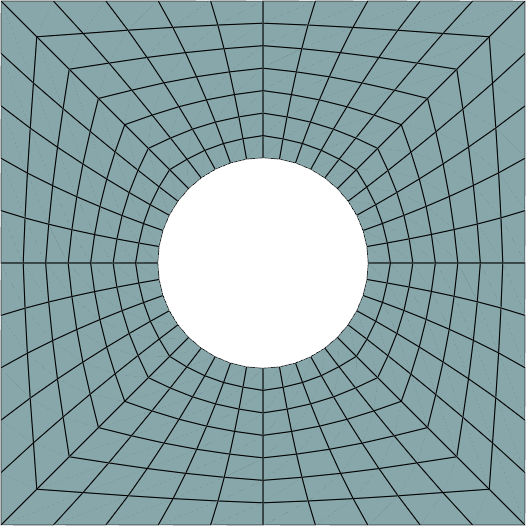
\includegraphics[width=0.65\textwidth]{../figures/beam/unit_cell.png}
    \end{center}
    \caption{Unit cell domain partition.}\label{fig:unit_cell_domain}
\end{figure}

\begin{figure}
    \begin{center}
        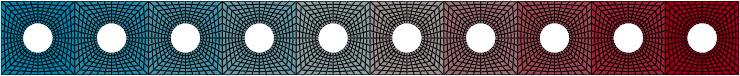
\includegraphics[width=0.95\textwidth]{../figures/beam/global_domain.png}
    \end{center}
    \caption{The partition of the global domain. The colors indicate the variation in Young's modulus for each subdomain.}\label{fig:global_domain}
\end{figure}

\subsection{Basis Construction}
For the beam problem, there are three oversampling problems to consider (left, inner, right).
For each of the associated parametric transfer operators, $n_{train}$ parameter samples are chosen, and
the range for each of these (fixed) transfer operators is approximated via random sampling. In
the sampling \textit{normal} or \textit{multivariate normal} distribution is used.
The range approximation of the $n_{train}$ transfer operators yields $n_{train}$ sets of
basis functions, which are further compressed via POD, to obtain the final parameter
independent basis functions (POD modes).

\subsubsection{Distributed approximate POD}

\begin{figure}[!htb]
\minipage{0.32\textwidth}
  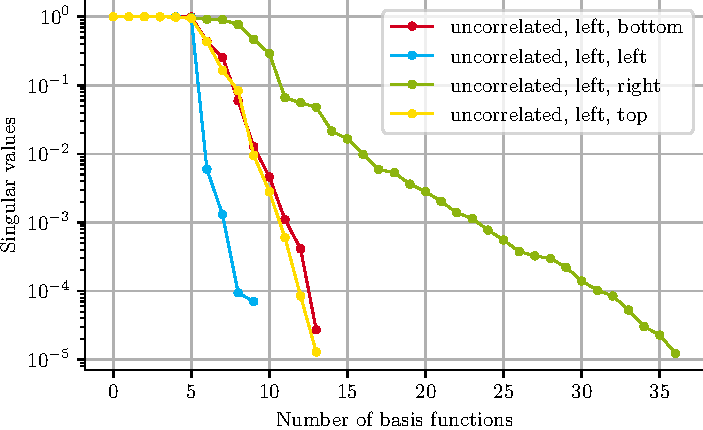
\includegraphics[width=\linewidth]{../figures/beam/fig_loc_svals_left.pdf}
  \caption{Singular valus left}\label{fig:loc_svals_left}
\endminipage\hfill
\minipage{0.32\textwidth}
  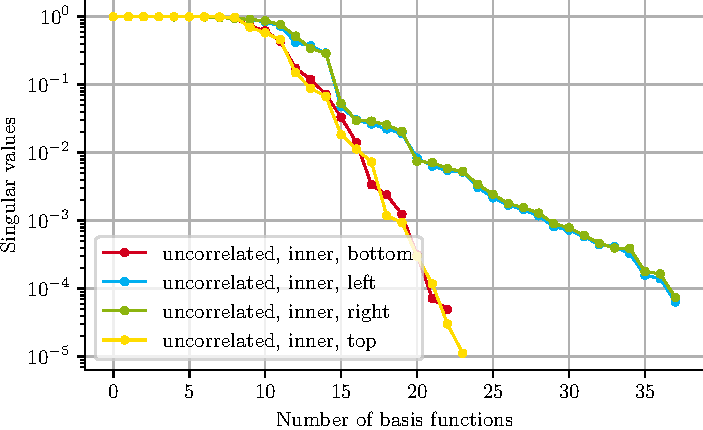
\includegraphics[width=\linewidth]{../figures/beam/fig_loc_svals_inner.pdf}
  \caption{Singular valus inner}\label{fig:loc_svals_inner}
\endminipage\hfill
\minipage{0.32\textwidth}%
  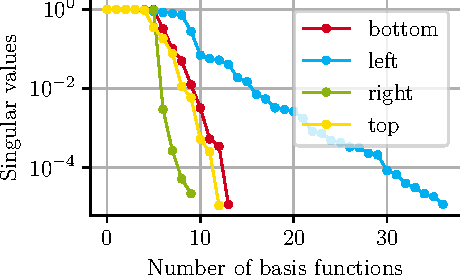
\includegraphics[width=\linewidth]{../figures/beam/fig_loc_svals_right.pdf}
  \caption{Singular valus right}\label{fig:loc_svals_right}
\endminipage
\end{figure}


% \subsubsection{Projection Error}
% The projection error is computed for a test set for each configuration that was computed
% using the FOM. Each test set has size $n_{test}$.

\begin{figure}[!htb]
\minipage{0.32\textwidth}
  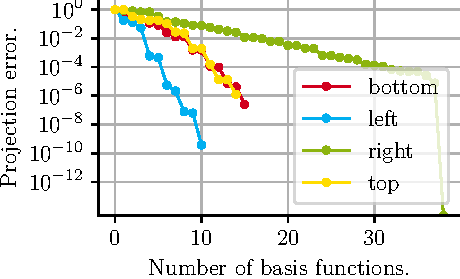
\includegraphics[width=\linewidth]{../figures/beam/fig_proj_error_left_hapod.pdf}
  \caption{Projection error hapod}\label{fig:proj_error_left_hapod}
\endminipage\hfill
\minipage{0.32\textwidth}
  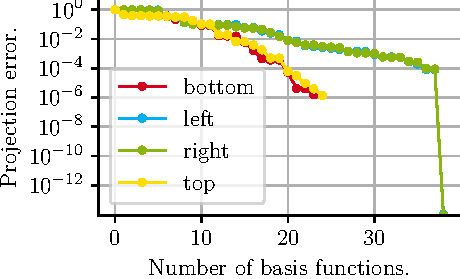
\includegraphics[width=\linewidth]{../figures/beam/fig_proj_error_inner_hapod.pdf}
  \caption{Projection error hapod}\label{fig:proj_error_inner_hapod}
\endminipage\hfill
\minipage{0.32\textwidth}%
  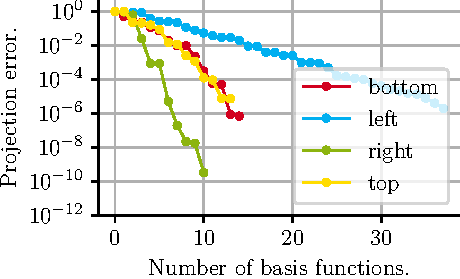
\includegraphics[width=\linewidth]{../figures/beam/fig_proj_error_right_hapod.pdf}
  \caption{Projection error hapod}\label{fig:proj_error_right_hapod}
\endminipage
\end{figure}

\subsubsection{Heuristic range finder}

\begin{figure}[!htb]
\minipage{0.32\textwidth}
  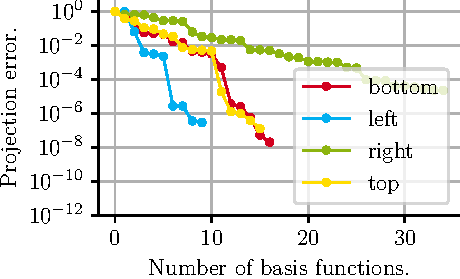
\includegraphics[width=\linewidth]{../figures/beam/fig_proj_error_left_heuristic.pdf}
  \caption{Projection error }\label{fig:proj_error_left_heuristic}
\endminipage\hfill
\minipage{0.32\textwidth}
  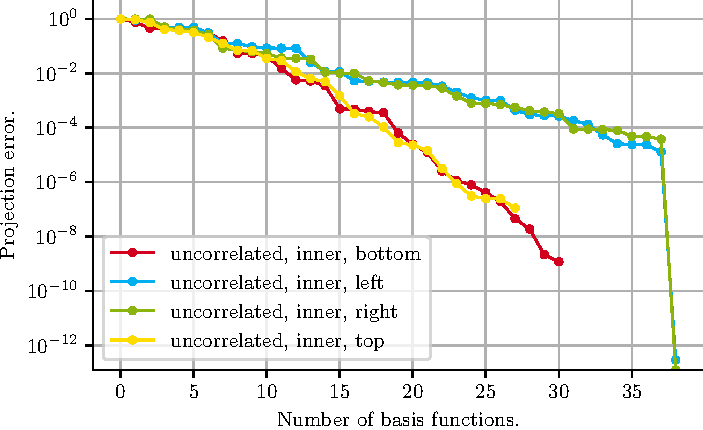
\includegraphics[width=\linewidth]{../figures/beam/fig_proj_error_inner_heuristic.pdf}
  \caption{Projection error }\label{fig:proj_error_inner_heuristic}
\endminipage\hfill
\minipage{0.32\textwidth}%
  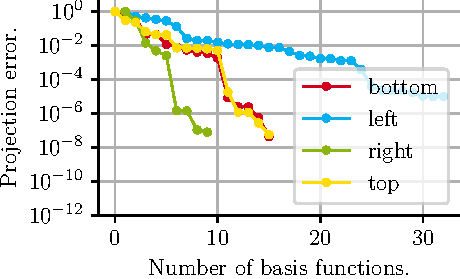
\includegraphics[width=\linewidth]{../figures/beam/fig_proj_error_right_heuristic.pdf}
  \caption{Projection error }\label{fig:proj_error_right_heuristic}
\endminipage
\end{figure}

\subsection{Localized ROM}

\begin{figure}[!htb]
    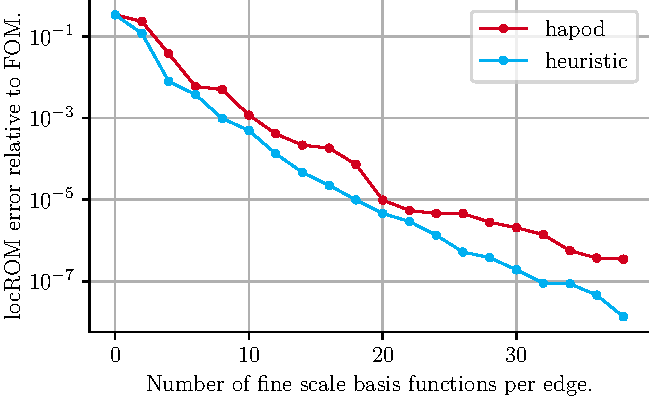
\includegraphics[width=\linewidth]{../figures/beam/fig_loc_rom_error.pdf}
    \caption{A really Awesome Image}\label{fig:loc_rom_error}
\end{figure}

\section{FORMAT OF REFERENCES}

References should be quoted in the text by superscript
numbers \cite{McQuerry18,nssga,Oden18} and grouped together at the end of the Full Paper in numerical order as shown in these instructions.

\section{CONCLUSIONS}

\begin{itemize}
\item[-] Full Papers in format for publication should be submitted electronically via the web page of the Conference, before \textbf{July 1st, 2024}. They must be converted to  Portable Document Format (PDF) before submission. The maximum size of the file is 4 Mb.
\end{itemize}

\begin{thebibliography}{99}
\bibitem{McQuerry18}  McQuerry, M. 2018. “Validation of a Clothing Heat Transfer Model in Nonisothermal Test Conditions.” J Test Eval 46, no. 1 (January/February): 1–7. http://doi.org/10.1520/JTE20170073

\bibitem{nssga}   National Stone, Sand, and Gravel Association (NSSGA). 2013. The Aggregates Handbook, 2nd ed. Englewood, CO: Society of Mining, Metallurgy, and Exploration.

\bibitem{Oden18}  Oden, C. P., C. L. Ho, and H. F. Kashani. 2018. “Man-Portable Real-Time Ballast Inspection Device Using Ground-Penetrating Radar.” In Railroad Ballast Testing and Properties, edited by T. Stark, R. Swan, and R. Szecsy, 77–104. West Conshohocken, PA: ASTM International. http://doi.org/10.1520/STP160520170023

\end{thebibliography}

\end{document}
